\chapter{Szczegóły Implementacyjne}
\label{chapter-4}

\section{Użyte narzędzia}

\noindent Projekt inżynierski został napisany zaimplementowany jako program komputerowy w języku python. Do realizacji zostały użyte głównie paczki:

\begin{itemize}
    \item numpy- paczka służąca do obliczeń naukowych. Udostępnia rozbudowane API do algebry liniowej i przetwarzania sygnałów.
    \item scipy- moduł umożliwiający obliczenia matematyczne i techniczne, w szczególności przetwarzanie sygnałów stosowane w tej pracy
    \item matplotlib- paczka służąca do wizualizacji danych.
    \item rir generator- moduł umożliwiający symulację odpowiedzi impulsowej pokoju
\end{itemize}

\noindent Więcej informacji można znaleźć w dokumentacji paczek \cite{numpy}, \cite{matplotlib}, \cite{rir} i \cite{scipy}.

\section{Metologia rozwoju programu}

\noindent Realizacja pracy była podzielona na stworzenie właściwego programu opisane szczegółowo w \ref{chapter-3} i na stworzenie generatora symulującego rzeczywisty sygnał mikrofonowy z dodatkiem zakłóceń.


W założeniach oprogramowanie miał mieć charakter obiektowy. Główne bloki zostały zaimplementowane jako klasy, które komunikują się między sobą za pomocą interfejsów. Takie rozwiązanie powoduje usystematyzowaną strukturę projektu i umożliwia łatwy rozwój oprogramowania w przyszłości. Przykładem jest implementacja algorytmu MUSIC. Klasa MUSIC dziedziczy po klasie abstrakcyjnej DOA. W ten sposób proste w przyszłości będzie dopisanie w programie innego algorytmu estymacji kierunku nadchodzenia fali jako innej klasy dziedziczącej po DOA. Poniżej przedstawiono diagram klas w konwencji UML \cite{uml}:

\begin{figure}[h]
    \centering
    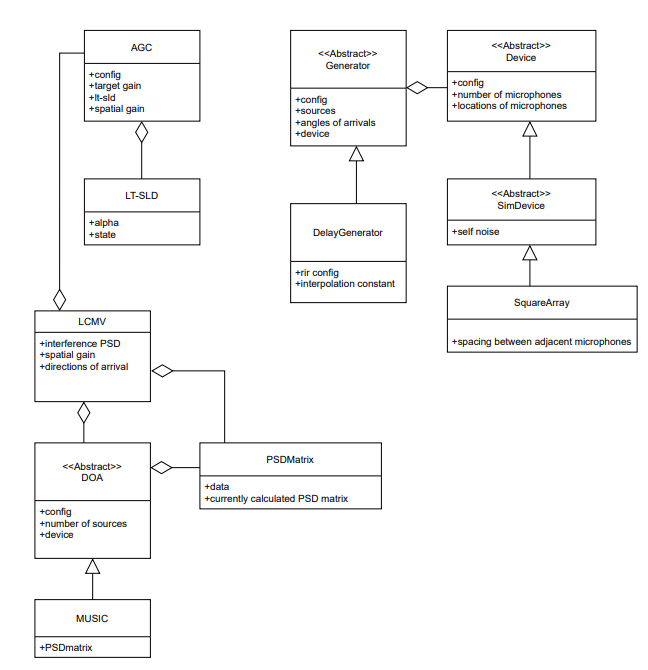
\includegraphics[width=\textwidth]{Images/uml.png}
    \caption{Diagram Klas}
    \label{fig:classes}
\end{figure}

\noindent W diagramie \ref{fig:classes} nie zawarto metod klas, ponieważ schemat behawioralny został już przedstawiony w \ref{fig:block_diagram}.

\section{Generator}

Generator pełni ważną rolę w projekcie inżynierskim. Z tego powodu postanawia się poświęcić mu osobną sekcję w tekście. 

\noindent Generator przyjmuje jako wejścia następujący dane:

\begin{itemize}
    \item Obiekt macierzy mikrofonowej
    \item Sygnały dzwiękowe 
    \item Funkcję kąta w czasie
    \item Funkcję wzmocnienia w czasie
    \item Opcjonalnie informacje o geometrii pokoju i o tym czy symulacja pogłosu jest włączona
\end{itemize}

Schemat działania generatora jest względnie prosty. Przyjmuje się model przedstawiony w \ref{chapter-2}. Zakłada się, że sygnał wejściowy odpowiada wartości sygnału w punkcie $\bm{\mathrm{d}}_{0}$. Posiłkując się równaniami \ref{equation:2.4} i \ref{equation:2.5} można zapisać, że:

\begin{equation}
    \label{delay model}
    f_{l}(\bm{\mathrm{d}}_{m},t) = 
    f_{l}(\bm{\mathrm{d}}_{0},t-\tau)
\end{equation}

\noindent Gdzie $f_{l}(\bm{\mathrm{d}}_{m},t)$ to wymuszenie $l$-tej fali dzwiękowej w punkcie $\bm{\mathrm{d}}_{m}$. W takim układzie możliwe są bieżące zmiany opóźnienia bazując na pozycji źródła.

\noindent Generator umożliwia funkcję 